\documentclass{scrartcl}
\usepackage{german}
\usepackage[utf8]{inputenc}
\usepackage[german]{babel}

% zusätzliche mathematische Symbole, AMS=American Mathematical Society
\usepackage{amssymb}
\usepackage{amsmath}
% fürs Einbinden von Graphiken
\usepackage{graphicx}
\usepackage{verbatim}

% für Namen etc. in Kopf- oder Fußzeile
\usepackage{fancyhdr}

% erlaubt benutzerdefinierte Kopfzeilen
\pagestyle{fancy}

% um tabelle nach links zu schieben
\usepackage{changepage}

\usepackage{xcolor}

% Definition der Kopfzeile
\lhead{
\begin{tabular}{lllll}
Nils Hagner & 4346038 & Felix Karg & 4342014 \\
Michael Fleig & 4340085 & Anush Davtyan &4368689
\end{tabular}
}
\chead{}
\rhead{\today{}}
\lfoot{}
\cfoot{Seite \thepage}
\rfoot{}

\begin{document}

\section*{Solutions for Excercise sheet 4}

\subsection*{Exercise 1 – LCS Syntax and Semantics}

	\begin{itemize}
		\item[(i)] LCS:
		\begin{figure}[h]
			\centering
			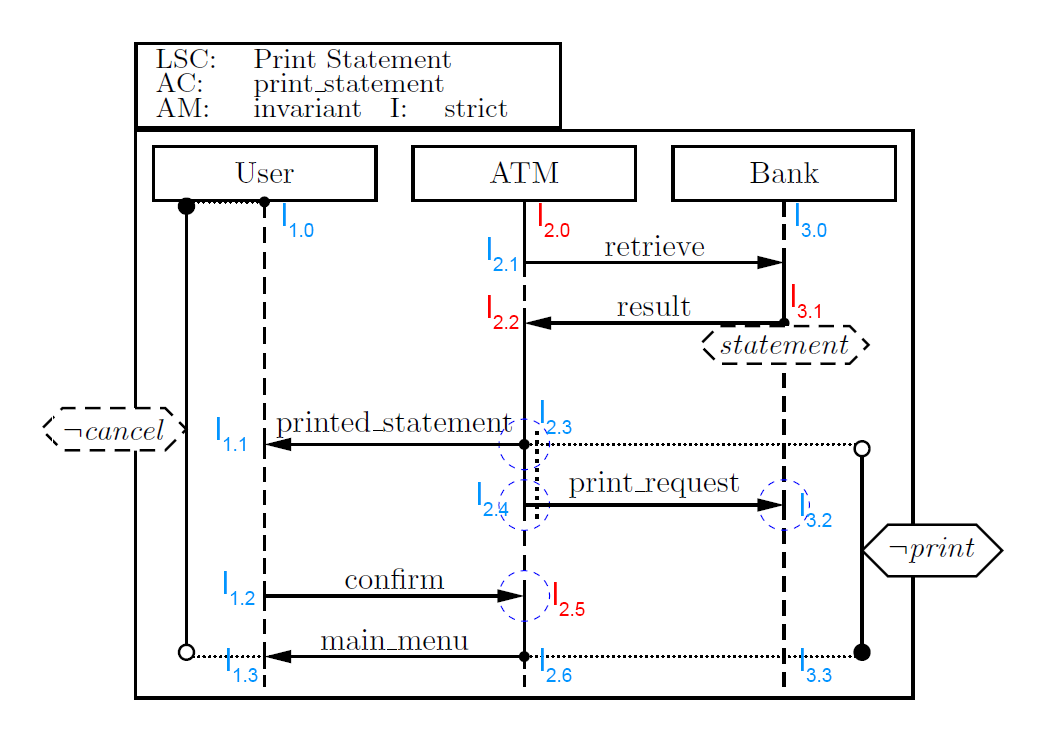
\includegraphics[width=\textwidth]{lcs.png}
		\end{figure}
		\begin{itemize}
			\item[a)] $\mathcal{L} = \{ 
				{\color{blue} l_{1.0}, l_{1.1}, l_{1.2}, l_{1.3},
			 	{\color{red} l_{2.0}}, l_{2.1}, {\color{red} l_{2.2}}, l_{2.3}, l_{2.4}, {\color{red} l_{2.5} }, l_{2.6},
			  	l_{3.0}, {\color{red} l_{3.1}}, l_{3.2}, l_{3.3}} \}$
		  	\item[b)] $ \mathcal{I} = \{ 
		  					\{ {\color{blue} l_{1.0}, l_{1.1}, l_{1.2}, l_{1.3}} \},
		  					\{ {\color{red} l_{2.0}}, {\color{blue} l_{2.1}}, {\color{red} l_{2.2}}, {\color{blue} l_{2.3}}, {\color{blue} l_{2.4}}, {\color{red} l_{2.5} }, {\color{blue} l_{2.6} } \},
		  					\{ {\color{blue} l_{3.0} }, {\color{red} l_{3.1}},  {\color{blue} l_{3.2}, l_{3.3} } \}
  						 \} $
		 	\item[c)] $ l_{2.4} \sim l_{3.3} $, $ l_{2.3} \preceq l_{2.5} $, $ l_{2.4} \preceq l_{2.5} $
		 	\item[d)] Msg: $ \{ (l_{2.1}, retrieve, l_{3.1}) \} $
		 	\item[e)] Inv: $ \{ {\color{red} l_{1.0}, \bullet, \neg cancel, l_{1.3}, \circ } \} $
		 	\item[f)] Cond: $ \{ {\color{blue} (\{ l_{3.2} \}, statement) } \} $
		\end{itemize}
		\pagebreak
		\item[(ii)] $ c_1 = \{ l_{1.0}, l_{2.0}, l_{3.0} \} $ \\
			$ c_2 = c_1 \cup \{ l_{2.1}, l_{3.1} \} $ \\
			$ c_3 = c_2 \cup \{ l_{2.2}, l_{3.2} \} $ \\
			$ c_4 = c_3 \cup \{ l_{2.3}, l_{1.1} \} $ \\
			$ c_5  = c_3 \cup \{ l_{2.4}, l_{3.3} \} $ \\
			$ c_6 = c_3 \cup \{ l_{2.3}, l_{1.1}, l_{2.4}, l_{3.3} \} $ \\
			$ c_7 = c_6 \cup \{ l_{1.2}, l_{2.5} \} $ \\
			$ c_8 = c_7 \cup \{ l_{2.6}, l_{1.3} \} $ \\
			
			\begin{figure}[h]
				\caption{Büchi automaton}
				\centering
				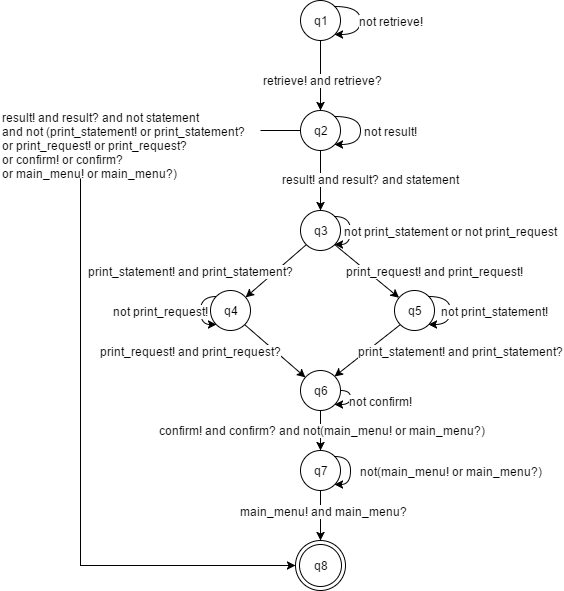
\includegraphics[width=\textwidth]{automaton.png}
			\end{figure}
		
		\item[(iii)] Strictness conditions omitted for readability.\\
			\begin{itemize}
			
		
			 \item[a)] $ \pi_{accept} = c_1 \xrightarrow{retrieve! \land retrieve?} c_2 \xrightarrow{result! \land result? \land statement} c_3 \xrightarrow{print-statement! \land print-statement?} c_4 \xrightarrow{print-request! \land print-request?} c_6 \xrightarrow{confirm! \land confirm?} c_7 \xrightarrow{main-menu! \land main-menu?} c_8$
			 
			 \item[b)] $ \pi_{exit} = c_1 \xrightarrow{retrieve! \land retrieve?} c_2 \xrightarrow{result! \land result? \land \neg statement} c_8 $ 
			 
			 \item[c)] $ \pi_{violate} = c_1 \xrightarrow{retrieve! \land retrieve?} c_2 \xrightarrow{result! \land result? \land statement} c_3 \xrightarrow{print-statement! \land print-statement?} c_4 \xrightarrow{print-request! \land print-request? \land print} illegal$
			\end{itemize}
	\end{itemize}


\end{document}
